\section{Durchführung und Aufbau}
\label{sec:Durchführung}
Zuerst werden die Magnetfelder zweier Spulen, einer langen und einer kurzen,
vermessen. Dafür wird eine longitudinale Hallsonde von einer Seite durch die Spule geführt und
nach jedem Zentimeter die magnetische Flussdichte gemessen.
Dabei werden je $\SI{5}{\centi\meter}$ vor und hinter der Spule gemessen sowie
jeden Zentimeter innerhalb der Spule.
\\
Als nächstes wird ein Helmholtzspulenpaar so aufgebaut, dass der Radius der
Spulen genau dem Abstand der Spulen zueinander entspricht.
Eine ähnliche Abbildung ist in Abbildung \ref{fig:helmskizze} dargestellt.
Die Flussdichte wird Zehn mal jeden halben Millimeter mit einer transversalen
Hallsonde gemessen, also
$\SI{0.5}{\centi\meter}$ in Summe. Außerdem wird die Flussdichte für
$\SI{10}{\centi\meter}$ außerhalb des Spulenpaares vermessen.
\\
Zuletzt wird eine Ringspule verwendet, welche an einer Stelle der Spule
ein Luftloch aufweist durch welches die Flussdichte mit Hilfe einer Hallsonde
in Abhängigkeit zur
Stromstärke gemessen wird.
Mit dieser Apparatur wird eine Hysterekurve aufgenommen.
Zuerst wird die Neukurve aufgenommen in dem die Stromstärke in einer
Schrittgröße von $\SI{1}{\ampere}$ von $0 - \SI{10}{\ampere}$ variiert und die
entsprechende Flussdichte notiert wird. Danach wird die Stromstärke wieder in
$\SI{1}{\ampere}$ Schritten auf Null reduziert. Nun muss die Stromstärke
umgekehrt werden und es wird erneut von $0 - \SI{10}{\ampere}$ gemessen. Dabei
muss der Punkt, an welchem die Flussdichte Null wird, genau abgelesen werden.
Danach wird die Spannung wieder bis nach $\SI{0}{\ampere}$ gemessen und die
Stromstärke wieder umgekehrt. Der zweite Punkt des Nulldurchganges der
Flussdichte wird wieder genau abgelesen und die Flussdichte wird wieder bis
$\SI{10}{\ampere}$ vermessen.
Damit erhällt man eine komplette Hysteresekurve.

\begin{figure}
  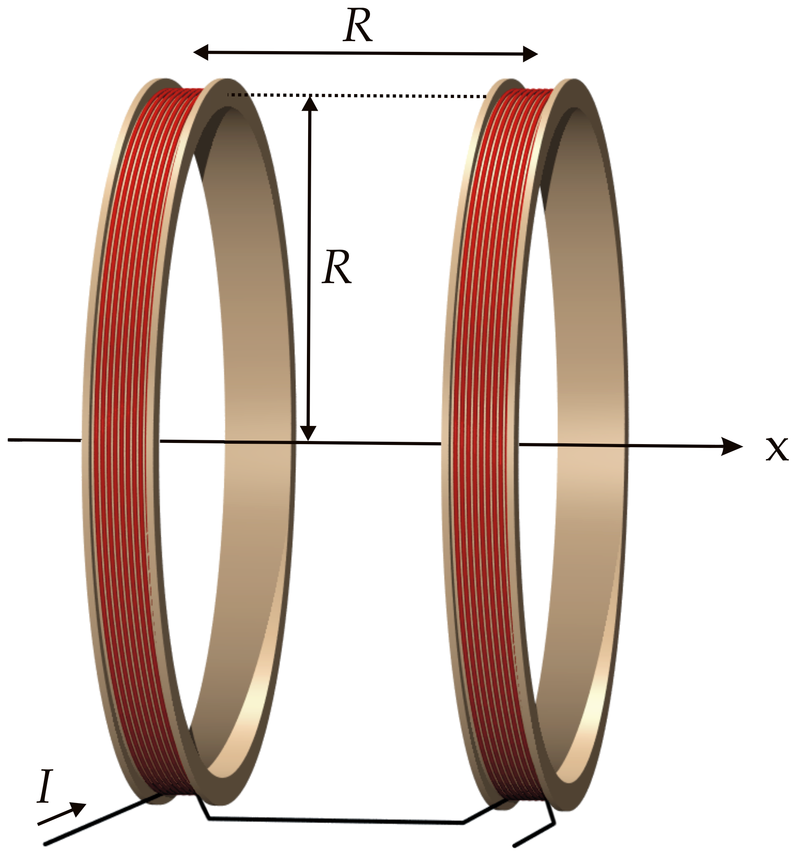
\includegraphics[height=9cm]{content/helmi.png}
  \caption{Schematische Abbildung eines Helmholtzspulenpaares\cite{Helmskizze}.}
  \label{fig:helmskizze}
\end{figure}
